\section{正 winding 模型の regular wall の保周期的な整形}
\label{we:section}

第\ref{tp:section}節の chosen graph form に対する比較を、central component wall の近傍へ延長する。
新しい foliation は fixed nonzero slice で旧 foliation と Hamiltonian 同値であり、
指定した whole focus end と whole saddle fiber の近傍では同一である。
従って新しい critical points を作らず、全 marked actions も保つ。
Central slice の通常の elliptic collapse と、nonzero slice に新たな singularity を作ることを区別する。

\subsection{Regular lower annulus の action}

標準一次共役因子模型で
\[
 H=P_x+P_y,\quad J=P_y-P_z,\quad u=P_y,\quad
 W=\bar X_1X_2X_3,\quad Q=|W-c|^2
\]
とする。Dense torus の周期 $1$ の角を
\[
 \alpha=\theta_1,\quad \beta=-\theta_3,\quad
 \phi=-\theta_1+\theta_2+\theta_3
\]
と変換すれば integral unimodular であり、
\begin{equation}\label{we:primitive}
 \lambda_{\rm std}=H\,d\alpha+J\,d\beta+u\,d\phi,\qquad
 \omega_{\rm red}=du\wedge d\phi
\end{equation}
となる。固定した $(h,j)$ に対し
\[
 L=\max(0,j),\quad
 f(u)=\frac{\sqrt{(h-u)u(u-j)}}{\pi^{3/2}},
 \quad L<u<u_1,\quad F=f(u_1)
\]
を lower radial branch と書く。
$F>2c$ とし、$c^2<q<(F-c)^2$ とする。
Lower reduced circle は global graph
\begin{equation}\label{we:graph}
 u=U(h,j,q,\phi)
 =f_{h,j,-}^{-1}\left(c\cos(2\pi\phi)
       +\sqrt{q-c^2\sin^2(2\pi\phi)}\right)
\end{equation}
であり、$U_q>0$ である。
従って
\begin{equation}\label{we:action}
 I(h,j,q)=\int_0^1U(h,j,q,\phi)\,d\phi
\end{equation}
は smooth で $I_q>0$ を満たす。

\begin{lemma}[壁を含む regular annulus]\label{we:annulus}
Compact parameter rectangle $R$ 上で smooth functions $b_-<b_+$ が
\[
 L<b_-<b_+<u_1,\qquad f(b_-)>2c,\qquad F-f(b_+)>2c
\]
を一様に満たすとする。
このとき $c^2<q_a<q_b<(F-c)^2$ を smooth に選んで
\[
 U(h,j,q_a,\phi)<b_-<b_+<U(h,j,q_b,\phi)
\]
を全 $\phi$ について成立させられる。
従って $[b_-,b_+]$ 内の全 constant circles は、
whole focus end と whole saddle fiber の間の同じ regular annulus に入る。
\end{lemma}
\begin{proof}
例えば
\[
 q_a=\frac{c^2+(f(b_-)-c)^2}{2},\qquad
 q_b=\frac{(f(b_+)+c)^2+(F-c)^2}{2}
\]
と置く。$u=b_-$ 上の $Q$ の最小値は $(f(b_-)-c)^2$、
$u=b_+$ 上の最大値は $(f(b_+)+c)^2$ であり、lower branch の単調性を使えばよい。
\end{proof}

\subsection{Hamiltonian straightening}

\begin{theorem}[全作用を保つ相対整形]\label{we:straightening}
補題\ref{we:annulus}の条件の下で、$H,J$ と可換な compactly supported
Hamiltonian isotopy $\psi_t$ があり、次を満たす。
保護する focus end の window は $q<q_a$、saddle neighborhood は $q>q_b$ に取る。
Strict gaps により、それぞれ whole singular fiber を含むこのような近傍を選べる。
あらかじめ指定した end window を点ごとに保つ場合には、
その window と support annulus の非交差を追加の相対条件とする。
\begin{enumerate}
\item Support は上記 regular lower annulus に入り、whole focus end と
  whole saddle fiber の共通近傍では $\psi_t=\mathrm{id}$ である。
\item $Q^\natural=Q\circ\psi_1^{-1}$ と置けば、$b_-<u<b_+$ の full neighborhood で
  \begin{equation}\label{we:toric}
   Q^\natural=\mathcal Q(H,J,u),\qquad I(H,J,\mathcal Q(H,J,u))=u.
  \end{equation}
  従ってその葉は full toric moment fibers である。
\item $H,J$、connected-fiber quotient、全 singularity types、
  transported marked actions と period lattice を保つ。
  特に新しい saddles、minima、degenerate critical points は作らない。
\end{enumerate}
$R$ を少し大きい rectangle の内部に取れば、その外周に恒等な isotopy として構成できる。
この場合、toric straightening の結論を主張する parameter set は内側の $R$ である。
\end{theorem}

\begin{proof}
\[
 U_t=(1-t)U+tI
\]
と置けば $(U_t)_q=(1-t)U_q+tI_q>0$ であり、$\int_0^1U_t\,d\phi=I$ である。
従って moving annulus 上で $u=U_t(q,\phi)$ の smooth inverse
$q=q_t(h,j,u,\phi)$ が存在する。

$I(q_a)<b_-<b_+<I(q_b)$ である。
少し大きい action interval $B(h,j)$ を選び、$[b_-,b_+]\Subset B$ とし、
その中の全 constant circles が元の regular annulus に入るようにする。
具体的には、下端を $f_-^{-1}(c+\sqrt{q_a})$ と $b_-$ の間、
上端を $b_+$ と $f_-^{-1}(\sqrt{q_b}-c)$ の間に取れる。
$\eta(h,j,I)$ を $[b_-,b_+]$ の近傍で $1$、$B$ の外で $0$ となる smooth cutoff とする。
周期関数
\[
 k(h,j,q,\phi)=\int_0^\phi
 \bigl(U(h,j,q,s)-I(h,j,q)\bigr)\,ds
\]
を定義する。Integrand の一周期の積分は零なので $k$ は well-defined である。
Moving annulus 上で
\begin{equation}\label{we:hamiltonian}
 K_t(H,J,u,\phi)=
 \eta(H,J,I(H,J,q_t))\,k(H,J,q_t,\phi)
\end{equation}
とし、その外では零とする。
Cutoff は moving annulus の両端で零なので smooth に延びる。
Support において $U(q,\phi)$ と constant $I(q)$ はともに元の protected annulus 内にある。
よってその convex combination $U_t$ もそこに入り、
$K_t$ の support は固定された compact regular annulus に一様に含まれる。
必要なら $H,J$ の少し大きい rectangle で parameter cutoff を掛ける。

規約 $\iota_{X_K}\omega=-dK$ の下で、graph $u=U_t(q,\phi)$ 上の normal velocity は
\[
 X_K^u-(U_t)_\phi X_K^\phi
 =-\partial_\phi(K_t|_{\text{graph }q}).
\]
$\eta=1$ の inner family では、右辺は $I-U=\partial_tU_t$ である。
従って flow は graph $U_0(q,\phi)$ を $U_t(q,\phi)$ へ送り、
時刻 $1$ には $u=I(q)$ へ送る。
$H,J$ derivatives は $\alpha,\beta$ の動きを追加するだけであり、$H,J$ 自体は一定である。
これで式\eqref{we:toric}を得る。

Support は prescribed singular fibers とその近傍から離れている。
新しい系は旧系の Hamiltonian conjugate なので、critical set と critical values は変更されず、
connected fibers と quotient は $\psi_1$ で同定される。
最後に
\[
 \frac{d}{dt}\psi_t^*\lambda_{\rm std}
 =d\left(\psi_t^*(\lambda_{\rm std}(X_{K_t})-K_t)\right)
\]
だから $\psi_t^*\lambda_{\rm std}-\lambda_{\rm std}$ は exact である。
従って全 closed marked cycles の actions が厳密に保たれる。
\end{proof}

\begin{remark}
Regular annulus 内では foliation を変更するが、protected focus end と saddle neighborhood では
点ごとに恒等である。従って、既に接いだ curve block を変えず wall の内部だけを処理できる。
単なる位相的な isotopy ではなく、actual symplectic form に対する Hamiltonian isotopy を使っている。
また annular insertion の primitive $s\lambda_{\rm std}+b\,d\theta_1$ についても、
support は $X_1\ne0$ にあり、isotopy による closed form $d\theta_1$ の変化は exact である。
従って affine offset を含む marked periods も変えない。
\end{remark}

\begin{remark}[Radial replacement の作用補正]\label{we:action-correction}
保周期的な radial integral は一般に $f(u)^2+c^2$ とは異なる。
$h,j,u$ が compact regular band にあるとして $c\to0$ とすると、
$v=f_-^{-1}$ に対して
\[
 I(q)=v(\sqrt q)+\frac{c^2}{4}
 \left(v''(\sqrt q)-\frac{v'(\sqrt q)}{\sqrt q}\right)+O(c^4)
\]
であり、従って
\[
 \mathcal Q(h,j,u)
 =f(u)^2+\frac{c^2}{2}
 \left(1+\frac{f(u)f''(u)}{f'(u)^2}\right)+O(c^4).
\]
これは式\eqref{we:graph}を $c$ で展開して一周期平均を取り、
$I(q)=u$ を解けば得られる。Odd powers は $\phi\mapsto\phi+1/2$ の対称性で消える。
単に角依存項を cutoff して $f^2+c^2$ に置換する操作には、この作用補正は含まれない。
\end{remark}

\subsection{一つの component wall}

$M_1=P_x-P_y=H-2u$ とし、wall $M_1=e_1$ の位置を
$b_1(h,j)=(h-e_1)/2$ とする。
一壁版では $R\Subset\{j<e_2\}$ として、
この hyperplane が実際の $D_i$--$D_j$ wall になる領域を扱う。
Compact $R$ 上で
\begin{equation}\label{we:onewall-gap}
 L<b_1<u_1,\qquad 2c<\min\{f(b_1),F-f(b_1)\}
\end{equation}
が一様に成立するとする。
$b_\pm=b_1\pm\delta$ を十分小さい $\delta>0$ で選べば
定理\ref{we:straightening}が適用できる。
新しい fibration は wall の full neighborhood で
$Q^\natural=\mathcal Q(H,J,P_y)$ となり、collapse circle $M_1$ は全 fibers を保つ。

これは invariant Hamiltonian が symplectic cut の両側へ降下する通常の原理に適合する
\cite[\S1.1, Remarks 1.2 and 1.6]{lerman-cut-local}。
ここではその原理の引用だけで relative end data を省略せず、
必要な invariance を Hamiltonian construction で作った。
$(H,J,u)$ は full moment lattice の integral basis であり、
$M_1=H-2u$ は primitive である。従って central collapse は通常の smooth elliptic collapse である。
Chosen pair $(H,J)$ の wall 上での有限 kernel と、ambient orbifold singularity を混同してはいけない。

\subsection{二つの位相を持つ壁の同時処理}

$M_{13}=P_x-P_z=H+J-2u$ とし、
$b_{13}(h,j)=(h+j-e_1-e_2)/2$ とする。
各 wall の collapse circle に関する $W$ の weight は
\[
\begin{array}{c|c|c}
\text{wall}&\text{generator}&\text{weight}\\ \hline
M_1=e_1&(1,-1,0)&-2\\
M_{13}=e_1+e_2&(1,0,-1)&-2\\
J=e_2&(0,1,-1)&0 .
\end{array}
\]
最後の wall については元から $W$ が invariant である。

両方の $b_1,b_{13}$ が一様に $L<u<u_1$ に入り、
\begin{equation}\label{we:twowall-gap}
 2c<\min_{r\in\{1,13\}}\{f(b_r),F-f(b_r)\}
\end{equation}
を満たせば、両者を含む smooth enclosing interval $[b_-,b_+]$ を選べる。
例えば midpoint と $\sqrt{((b_1-b_{13})/2)^2+\delta^2}$ を使えば、
$j=e_2$ で両者が一致する場合も smooth である。
Strict inequalities と compactness により、小さい $\delta$ で補題\ref{we:annulus}が適用できる。
一つの straightening により、両 walls とその交わりで同時に toric になる。
Sequential な二つの isotopies を使わないので、$j=e_2$ の整合問題は生じない。

例えば
\[
 h_{\min}>e_1+2\max_R\max(0,j),\qquad
 h_{\min}>e_1+e_2+\max_R|j|
\]
を strict margin 付きで課せば、両 walls は lower pole から離れる。
また $u_1>h/2$ と $u_1>(h+j)/2$ より maximum より下にある。
従って十分小さい $c>0$ で式\eqref{we:twowall-gap}が成立する。
これは $j=0$ と $j=e_2$ の双方を含む window でも実現できる。

\begin{figure}[htbp]
\centering
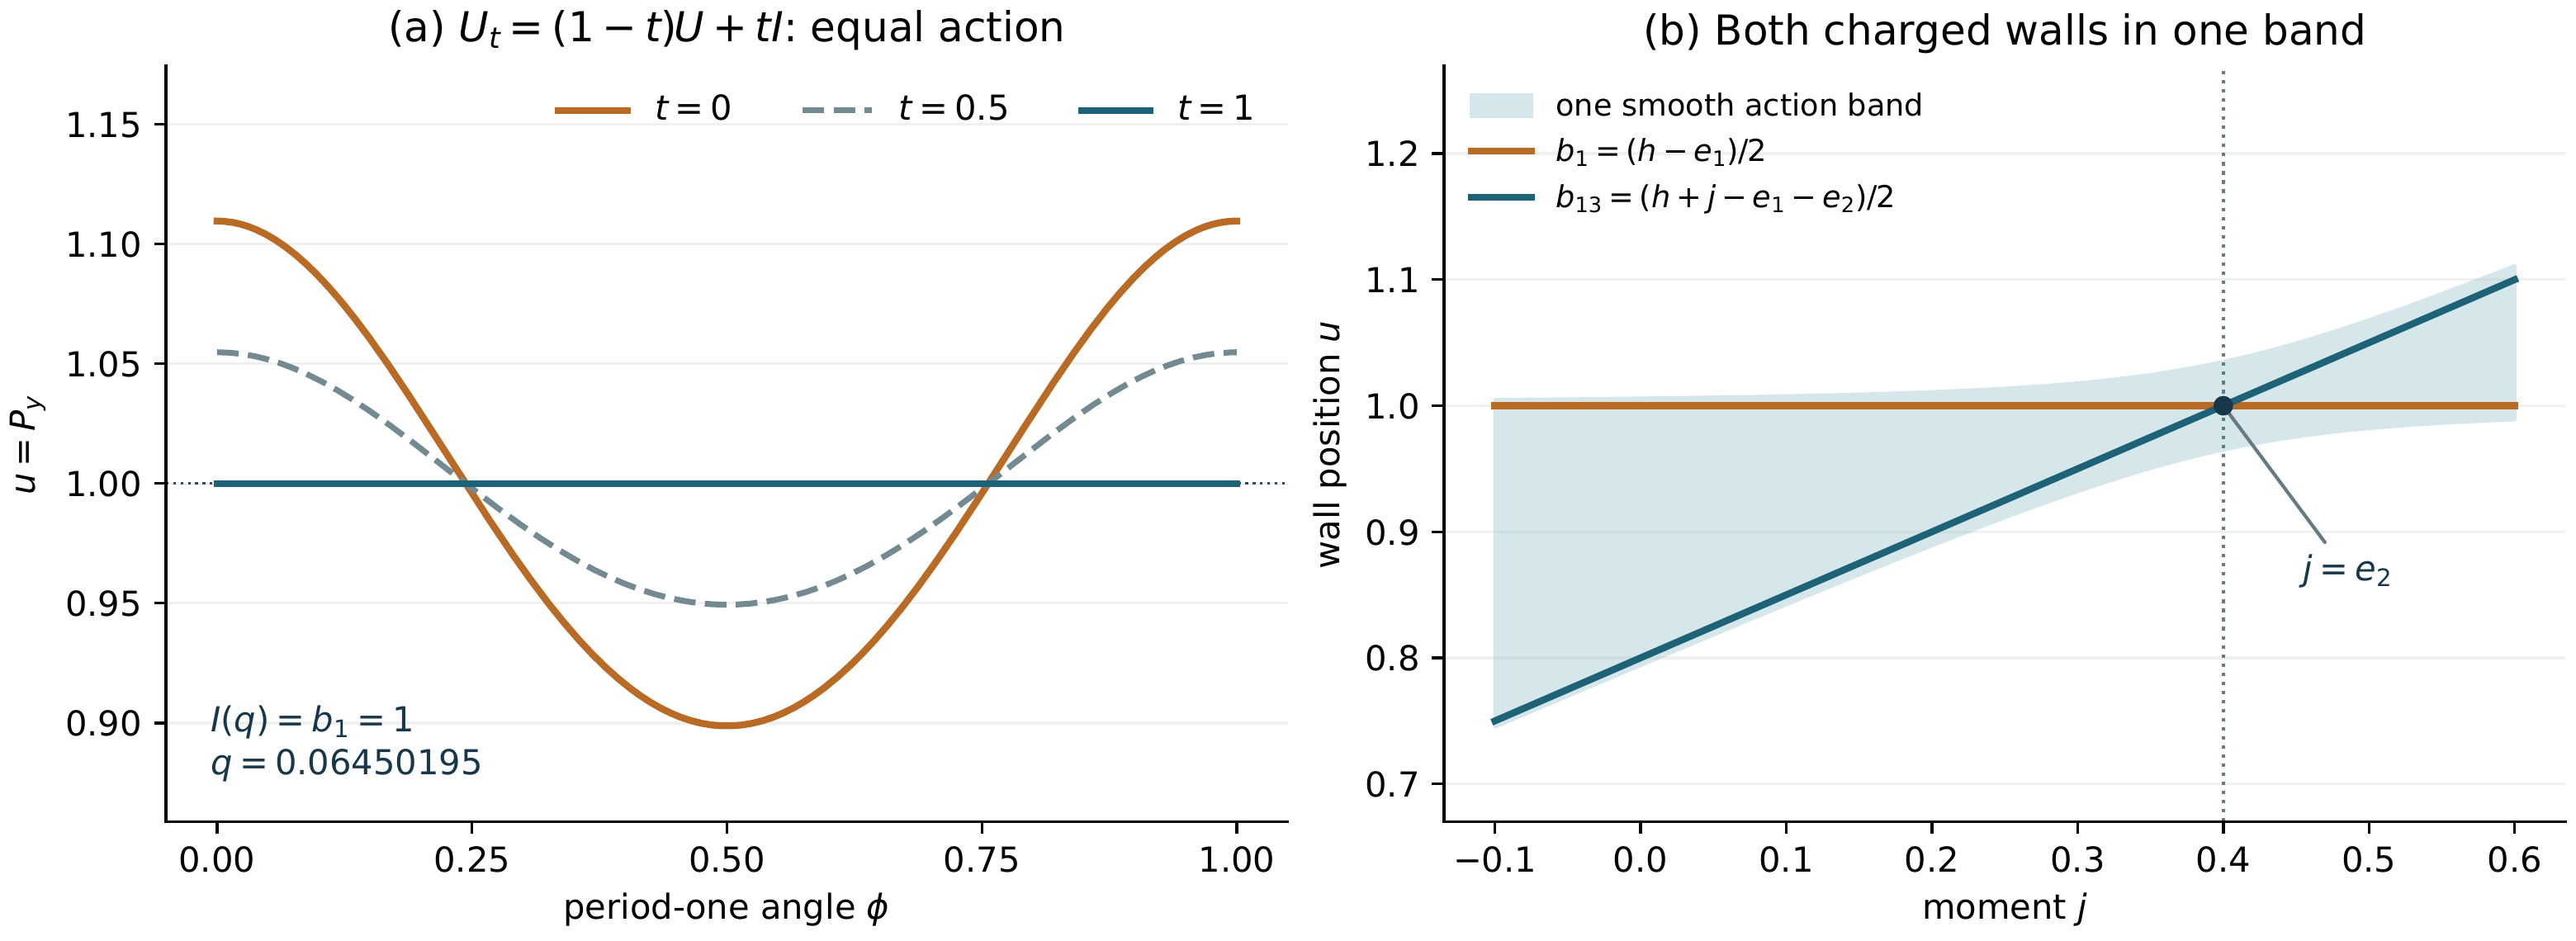
\includegraphics[width=\textwidth]{wall_straightening_geometry.png}
\caption{作用を保つ整形と二壁の同時処理。
(a) $h=3,j=0,c=0.02,e_1=1$ に対し、$I(q)=b_1=1$ を満たす
level graph を、その平均を変えず水平な円へ動かす。
(b) 同じ $h,c,e_1$ と $e_2=0.4$ について、二つの wall positions を
一つの smooth band に入れる。$j=e_2$ での一致でも band は滑らかである。
数値図は定理\ref{we:straightening}の構成を示すもので、存在証明は本文による。}
\label{we:figure}
\end{figure}

\subsection{Chosen resolved family 上の actual extension}

正の実 parameter $\tau>0$ に沿って考える。
Exact radial map $\Phi_\tau$ により $\psi_t$ を $\Omega_\tau$ 上の Hamiltonian isotopy へ運び、
\[
 (H_\tau,J_\tau,Q_\tau^\natural)
 =(H,J,Q^\natural)\circ\Phi_\tau
\]
とする。Whole focus end と whole saddle neighborhood は元の actual fibers のままである。

Central extension には isotopy 自体を $\tau=0$ へ延ばす必要はない。
まず標準空間上の一つの smooth function $Q^\natural$ を作っている。
これは $H,J$ invariant であり、修正領域では $G(H,J,u,\phi)$ と書ける。
修正の support は $P_xP_yP_z>0$ の compact regular region にあり、
wall shell では $G=\mathcal Q(H,J,u)$ で角に依存しない。
これを以下の chart expressions と組み合わせる。

First chart $x=\tau X$ では
\[
 W=\bar Xyz\sqrt{q_X^Aq_y^Aq_z^A},
\]
\[
 q_X^A=|\tau|^2+|yz|^2+\frac{e_1}{\pi(1+|X|^2)}
                   +\frac{e_2|y|^2}{\pi(1+|Xy|^2)},\quad
 q_y^A=1+|Xz|^2+\frac{e_2|X|^2}{\pi(1+|Xy|^2)},\quad
 q_z^A=1+|Xy|^2
\]
であり、中央へ smooth に延びる。
Middle chart の $x\ne0$ では式\eqref{tp:Bmap}を使う。
Last chart $(x,y,U,w)$ では $t=xyU=\tau>0$ より
\begin{equation}\label{we:last-chart}
 W=\frac{\bar x}{x}\,w\,\frac{\sqrt{P_xP_y(1+|U|^2)}}{\pi}
\end{equation}
となる。この式は $x\ne0$ で $y=U=0$ の weight-zero wall にも smooth に延びる。
$P_y$ は正の項 $e_2/(1+|U|^2)$ を含む。

残る charged walls の近傍では $\mathcal Q(H,J,P_y)$ を用いる。
Full moments $P_i$ 自体は resolved total space 上で smooth なので、
この式は collapse locus へ smooth に延びる。
他の領域では chart expressions と $G$ の smoothness を用いる。
Local ambient extensions を partition of unity で貼れば、
real-ray family 上の同じ function の smooth extension が得られる。
$H,J$ の torus で平均化した partition を使える。
Central components 上の Poisson commutativity は smooth limit、または torus invariance による。

\begin{theorem}[Relative wall filling]\label{we:actual-filling}
式\eqref{we:onewall-gap}または二壁版\eqref{we:twowall-gap}の
compact open-window hypotheses の下で、chosen graph Kähler family 上に相対変更が存在し、
次を満たす。
\begin{enumerate}
\item 非零 slice では旧 system と exact Hamiltonian 同値であり、
 protected whole focus end と whole saddle neighborhood は点ごとに固定する。
\item 選んだ walls の full neighborhoods で toric であり、
 正実 $\tau$-ray に沿って両中央 components とその共通 divisor へ滑らかに延びる。
\item Central wall は primitive circle の ordinary elliptic collapse である。
 二つの charged walls が会う free-toric-stratum の seam では、
 primitive rank-two subtorus の collapse による elliptic--elliptic toric corner を得る。
\item Protected compact block の connected-fiber quotient は非零 slice で変更されない。
 既存の $D^2\times Y$ branching と compact focus end は保たれる。
\end{enumerate}
\end{theorem}

Compact block は第\ref{ai:compact-block}項と同じ lower/upper-leg 選択で取れる。
広い parameter window では upper boundary を $q_+(h,j)=F(h,j)^2+c^2$ とすれば、
$q_s<q_+<(F+c)^2$ が自動的に成り立つ。
Lower cutoff は $q_-<c^2$、upper-leg cutoff は $c^2<q_*<\min_Rq_s$ とする。
Straightening の support は lower regular annulus 内なので、
この compact block とその connected fibers を Hamiltonian conjugacy で追える。
$H,J$ faces を点ごとに固定する optional parameter cutoff を使った場合、
中央への全 wall extension は内側の parameter rectangle についての主張である。

\paragraph{Primitive と residue.}
Foliation の wall extension は、logarithmic primitive の smooth extension を意味しない。
Middle chart の nonzero slice では
\[
 \lambda_\tau=M_1d\theta_x+P_y d\theta_Y+P_zd\theta_z
\]
であり、中央 $D_j$ 側では $M_1=e_1+\rho_x$ となる。
従って $e_1d\theta_x$ の period は残る。
Hamiltonian 修正は primitive を exact form だけ変えるため、この residue を消さない。
Normal actions $M_1-e_1$ と $e_1-M_1$ は反対符号で接ぐが、
primitive の滑らかな延長とは別の主張である。

\paragraph{未処理の core.}
本定理の wall window は $P_xP_yP_z>0$ にある。
特に middle exceptional curve の locus
\[
 P_z=0,\qquad h=e_1+2j,\qquad 0\le j\le e_2
\]
には適用していない。そこでは wall と lower pole が衝突し、
regular-annulus straightening の前提が失われる。
第一の exceptional curve の $P_y=P_z=0,\ 0\le H\le e_1$ も本 window の外である。
従って全 exceptional chain の core の充填、全 artificial boundary の除去、
任意の global form と全 geometric corner faces の同時保持は依然として別の課題である。
今回完成したのは、whole focus end と true branch を保ったまま、
その間の actual regular component walls を通す相対 filling である。
